\subsection{Lab16: Transmisor AM}

%*********************
\begin{frame}{}

\pgfdeclareimage[width=\paperwidth,height=\paperheight]{bg}{imagenes/fondo_lab}
\setbeamertemplate{background}{\pgfuseimage{bg}}

\bfseries{\textrm{\LARGE Lab16\\ \Large Transmisor AM}}
\raggedright
\end{frame}
%*********************

\begin{frame}{Modulación de amplitud IQ}

\pgfdeclareimage[width=\paperwidth,height=\paperheight]{bg}{imagenes/fondo3}
\setbeamertemplate{background}{\pgfuseimage{bg}}

La modulación de amplitud (AM) funciona mediante la variación de la amplitud de la señal transmitida de alta frecuencia que varía en proporción con una señal que por naturaleza es de baja frecuencia. La señal de baja frecuencia es la información que se desea transmitir también llamada señal moduladora, usualmente se encuentra en el orden de los KHz y la señal de frecuencia alta se le llama portadora usualmente en el orden de los MHz. \\
\vspace{2mm}
Es una modulación digital que transmite dos mensajes independientes y está conformado por dos canales ortogonales $i(t)$ y $q(t)$ que pueden ser transmitidos simultáneamente. \\ \vspace{2mm}  
El canal $i(t)$ es la señal moduladora (entrada) que contiene la información y es la parte real para la transmisión, el canal $q(t)$ es la señal portadora que debe estar desfasada 90$^{\circ}$ de la señal moduladora y es la parte imaginaria para la transmisión\cite{Lecture9}.  




\end{frame}
%---------------------------------

\begin{frame}{Modulación de amplitud IQ}
\begin{wrapfigure}{l}{0.5\linewidth}
    \centering
    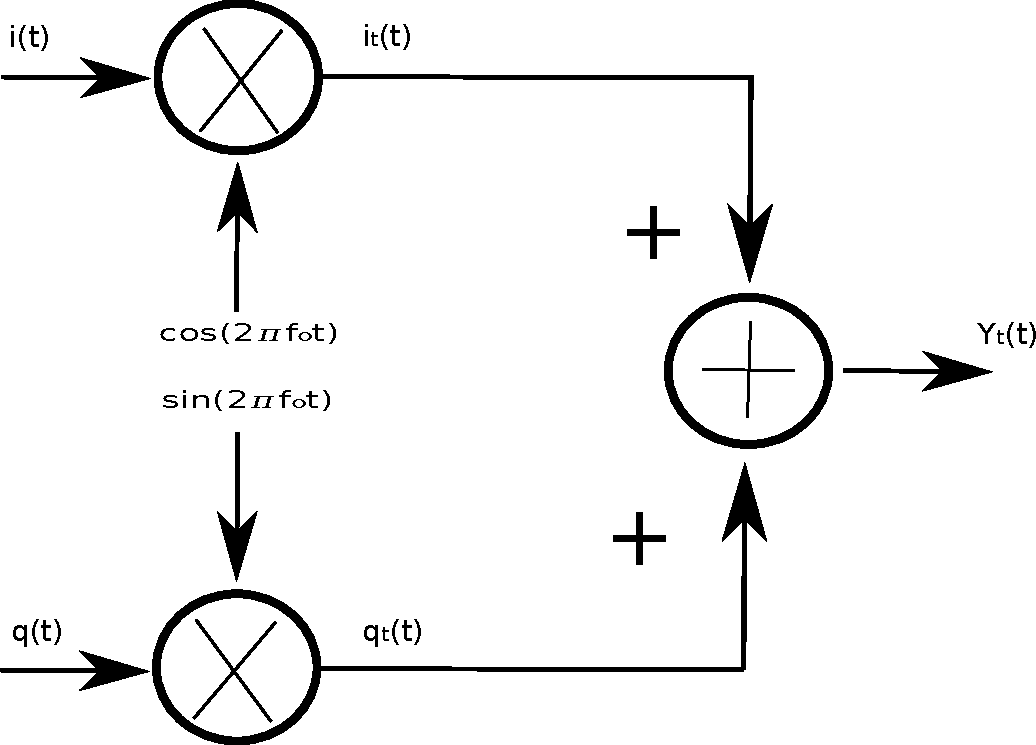
\includegraphics[width=0.5\textwidth]{parte3/lab15/pdf/lab15_1.pdf}
\end{wrapfigure}


Matemáticamente se expresa: \\\vspace{3mm}
\centering{
$i_t (t)=i(t)cos(2\pi f_0 t + 0^{\circ})$ \\ \vspace{2mm}
$q_t (t)=q(t)cos(2\pi f_0 t + 90^{\circ})=q(t)sin(2\pi f_0 t)$\\ \vspace{2mm}
$y_t (t)= \sqrt{i^{2} (t)+q^{2}(t)}cos(2\pi f_0 t + \theta(t))$\\ \vspace{2mm}
$\theta(t)=tan^{-1}\frac{q(t)}{i(t)}$\\\vspace{2mm}
$-180<\theta<180^{\circ}$\\ \vspace{2mm}}

\end{frame}
%---------------------------------

\begin{frame}{Modulación de amplitud IQ}

\begin{figure}[H]
\centering
\vspace{-3mm}
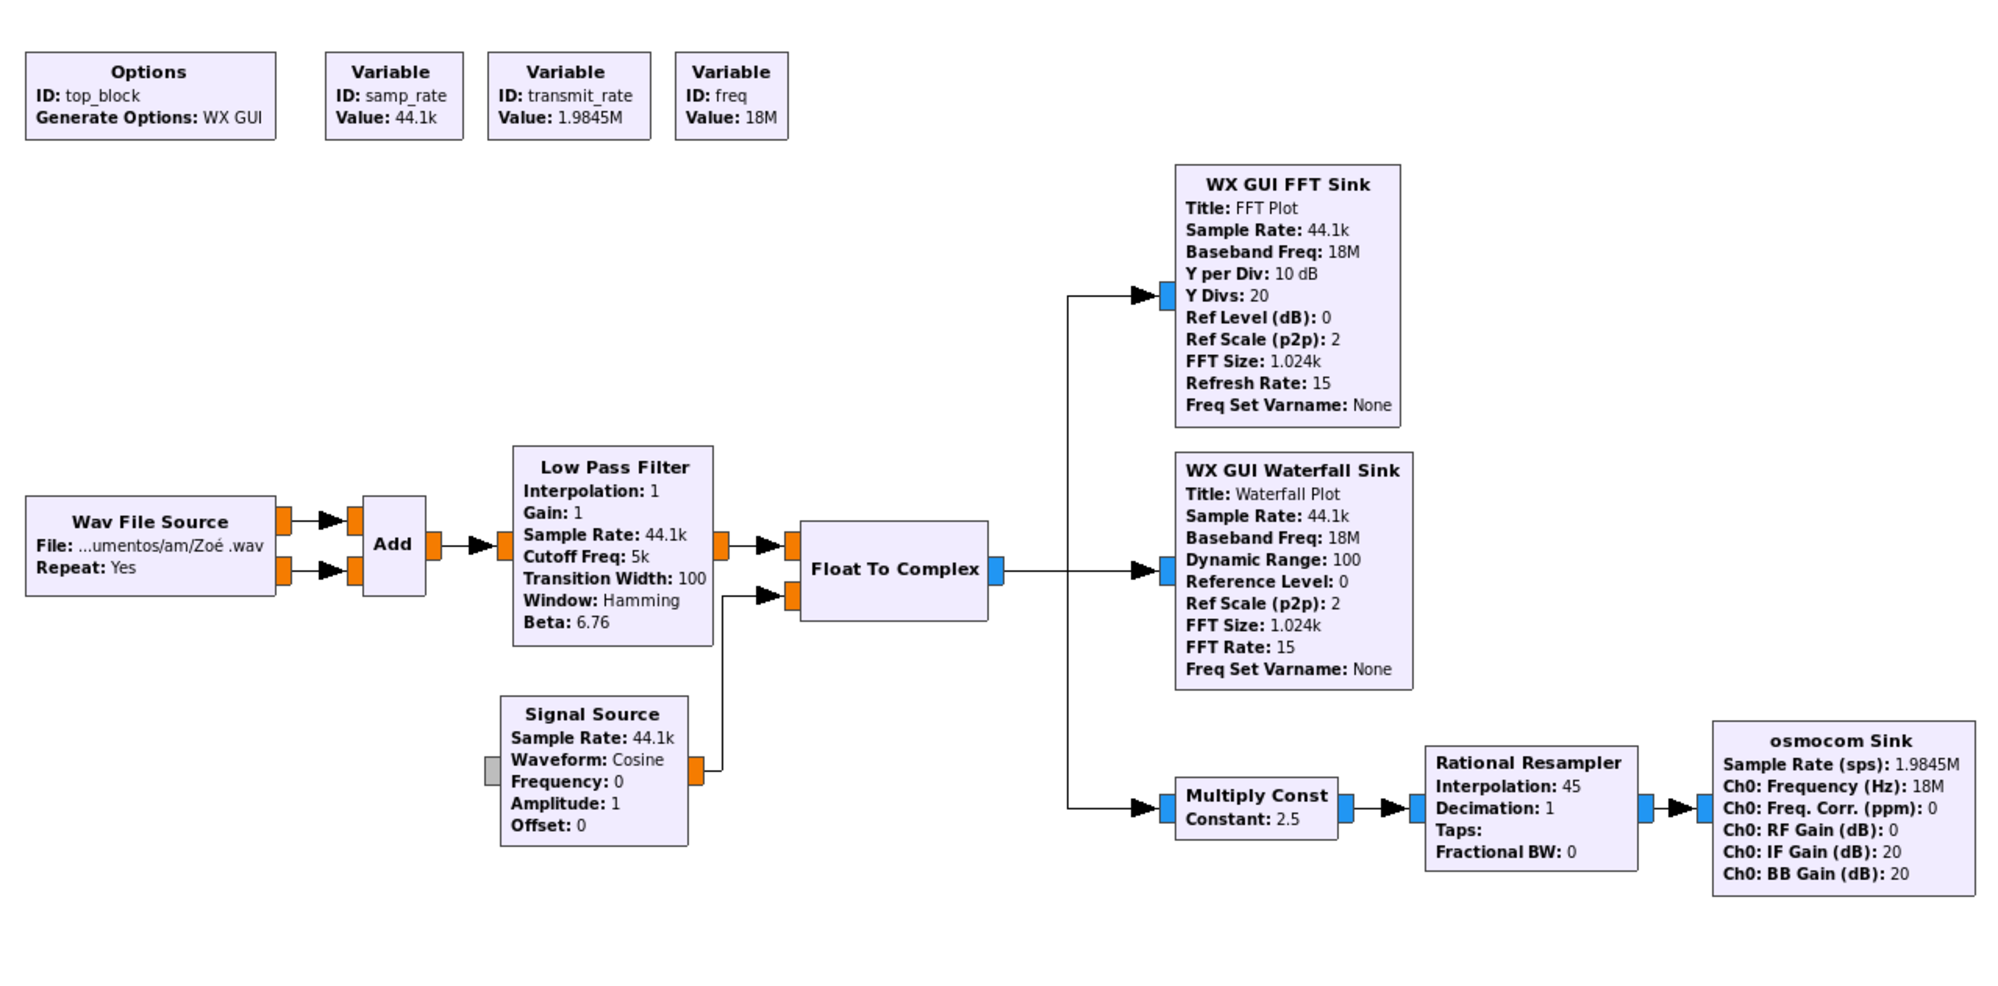
\includegraphics[width=\textwidth]{parte3/lab15/pdf/lab15_2.pdf}
\end{figure}

\end{frame}
%---------------------------------

\begin{frame}{Modulación de amplitud IQ}

\begin{figure}[H]
\centering
\vspace{-3mm}
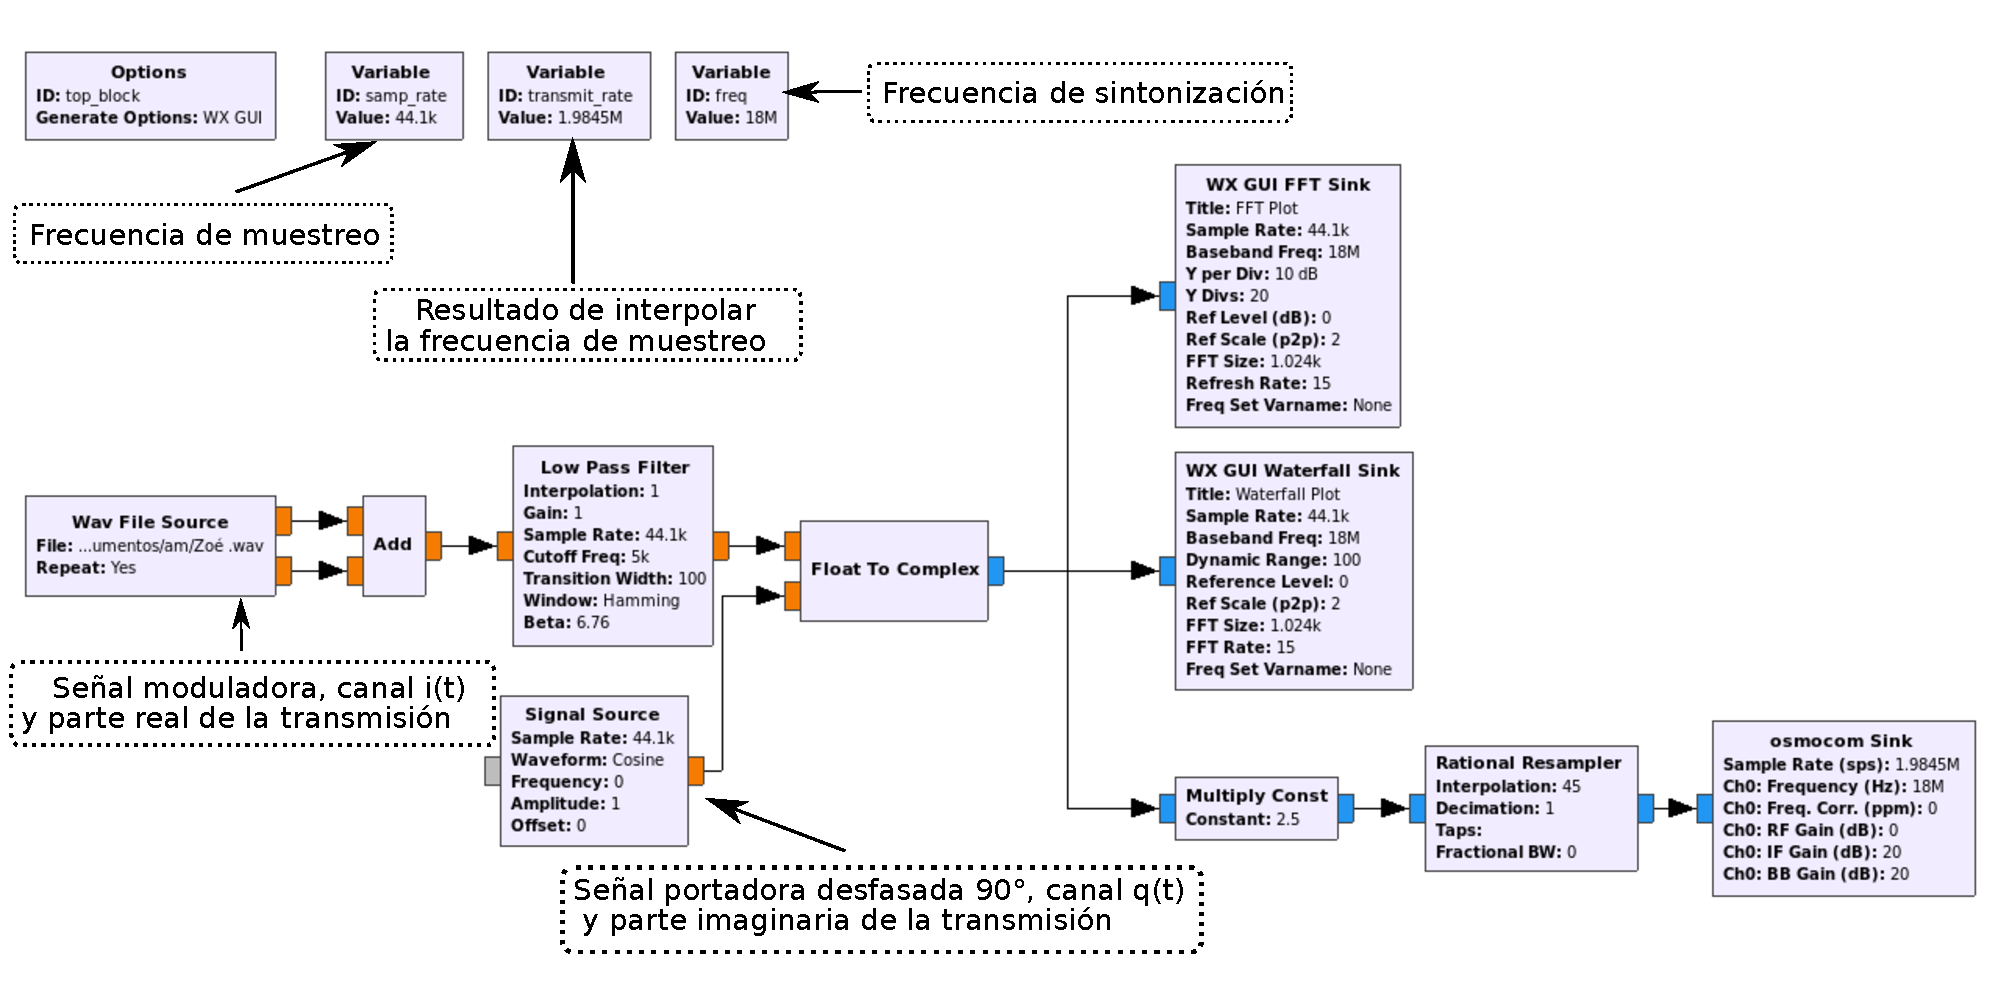
\includegraphics[width=\textwidth]{parte3/lab15/pdf/lab15_3.pdf}
\end{figure}

\end{frame}
%---------------------------------

\begin{frame}{Modulación de amplitud IQ}

\begin{figure}[H]
\centering
\vspace{-3mm}
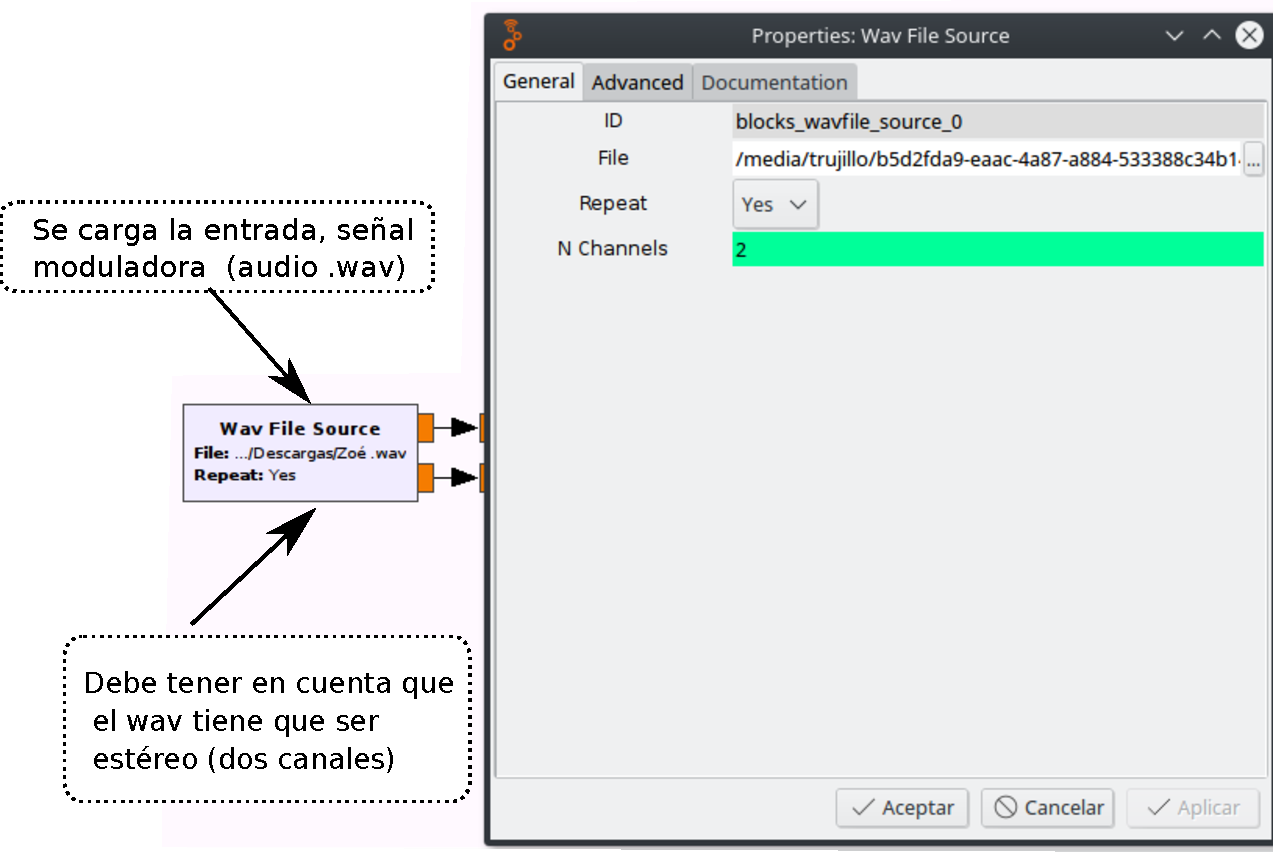
\includegraphics[width=.7\textwidth]{parte3/lab15/pdf/lab15_4.pdf}
\end{figure}

\end{frame}
%---------------------------------

\begin{frame}{Modulación de amplitud IQ}


El resultado de la modulación (señal modulada) no se puede observar en el dominio del tiempo ni de la frecuencia ya que el proceso de mezclado entre la señal portadora y moduladora se hace directamente con el HackRF, pero sí se puede observar el resultado de la unión entre la parte real e imaginaria (señal moduladora y portadora).  La frecuencia utilizada para mirar la señal en el dominio de la frecuencia (FFT) y el diagrama de cascada (espectrograma) es la sintonizada en el radio.

\end{frame}
%---------------------------------

\begin{frame}{Resultado}

\begin{figure}[H]
\centering
\vspace{-3mm}
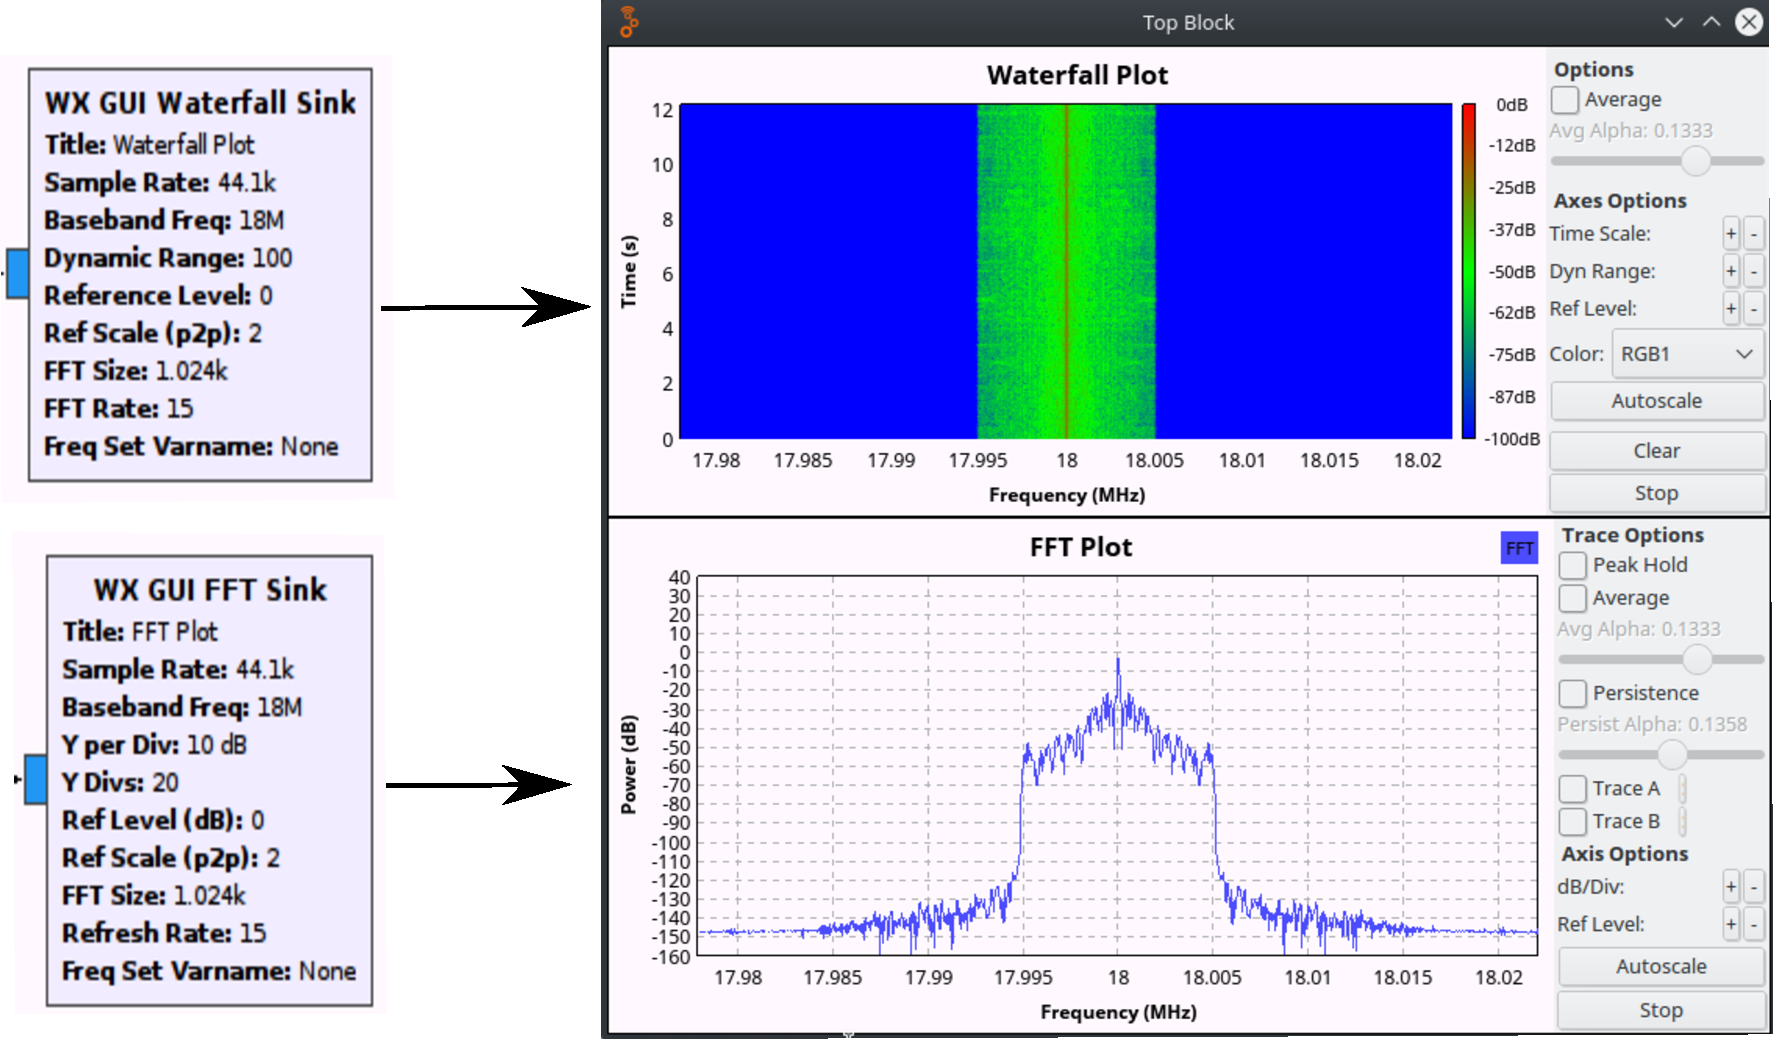
\includegraphics[width=\textwidth]{parte3/lab15/pdf/lab15_5.pdf}
\end{figure}

\end{frame}
%---------------------------------